\documentclass[runningheads]{llncs}

\usepackage{graphicx}
\usepackage{amsmath,amssymb}
\usepackage{booktabs}
\usepackage{listings}
\usepackage{xcolor}
\usepackage{tikz}
\usetikzlibrary{arrows.meta,positioning}
\usepackage[hidelinks]{hyperref}
\usepackage{cleveref}

\lstset{
  basicstyle=\ttfamily\small,
  numbers=none, frame=single, framesep=4pt,
  xleftmargin=1em, columns=fullflexible, keepspaces=true,
  language=C, showstringspaces=false, aboveskip=4pt, belowskip=4pt
}

\newcommand{\tool}{\textsc{VGuide}}
\newcommand{\cpa}{\textsc{CPAchecker}}
\newcommand{\llm}{DeepSeek\,V4\,Pro}

\begin{document}

\title{From Predicates to Ranking Functions:\\
LLM-Proposed, Engine-Validated Candidates for\\
CEGAR-Based Software Verification}

\author{Ssu-Wei Huang}
\institute{National Taiwan University, Taipei, Taiwan\\
\email{stanley.yellow1@gmail.com}}

\titlerunning{LLM-Proposed, Engine-Validated Candidates for CEGAR}
\authorrunning{Ssu-Wei Huang}

\maketitle

\begin{abstract}
Predicate abstraction with CEGAR and lasso-based termination both fail in the same place: a
loop needs a \emph{relational} fact---an invariant coupling variables, or a ranking measure
outside a fixed template---that no single counterexample path or synthesis family exposes.
We present \tool{}, an LLM oracle for \cpa{} governed by one rule: \emph{the model proposes,
the verifier decides, and nothing unvalidated reaches the engine}. The same
\emph{engine-validated candidate provider} shell covers two artifacts with \emph{different} gates.
For safety, loop predicates must pass contract and vocabulary checks and are injected only as
precision refinements at loop heads (monotone, so useless suggestions cannot yield a wrong
\textsc{True}); an SMT entailment tier was implemented but dropped after ablation hurt overall
performance. For termination, each ranking function and supporting invariant must discharge a
four-condition SMT proof on the lasso before use. On 764 SV-COMP Loops ReachSafety tasks,
\tool{} solves 29 more tasks than base predicate analysis in isolation ($224{\to}253$); on the
\texttt{svcomp26} portfolio a naive deployment adds $+7$ ($486{\to}493$); a stock-first schedule
reaches \textbf{505} ($+19$), while adding an early peel trigger trades nine wins for nine losses
at the same solve count (\Cref{tab:safety}). Termination adds four tasks ($80{\to}84$, 0 lost, 0 wrong) on 146
integer-termination benchmarks. We report these gains together with their limits: most
residual safety tasks are nonlinear and out of scope for a linear predicate engine, and the
termination lift has a small, characterised ceiling.

\keywords{Software verification \and CEGAR \and Predicate abstraction \and
Termination \and Ranking functions \and Large language models.}
\end{abstract}

\section{Introduction}
\label{sec:intro}

Software verification has two mature loop-centric paradigms, both implemented at scale in
\cpa{}~\cite{cpachecker2011} and competitive at SV-COMP~\cite{svcomp2022}: predicate
abstraction with CEGAR~\cite{cegar2003,predabstraction1997,slam2002}, and termination via
lasso-based ranking-function synthesis~\cite{ranking2004,ultimate2014}. Each stalls when
the proof needs a relational fact the built-in search never surfaces. CEGAR refines from
Craig interpolants~\cite{interpolation2003} along \emph{one} spurious counterexample (CE)
path; if the invariant couples variables across iterations---$x+y=n$ in our running
example---interpolation discovers $\{y=n\}$, then $\{y=n-1\wedge x=1\}$, one conjunct per
unrolling, and the proof diverges. Termination analysis is symmetric: template synthesis
~\cite{ultimate2014} only finds measures in a fixed family and returns \textsc{Unknown} when
the true ranking function lies outside it.

\paragraph{A running example.}
\Cref{lst:example} is a counting loop. Safety needs the relational invariant $x+y=n$;
termination needs the ranking function $f=y$. Stock predicate CEGAR on this task times out
after 69 refinements at \textsc{Unknown}: the closing invariant never appears on any single CE
trace. A language model can plausibly \emph{name} both artifacts from loop structure alone.
The obstacle is trust---a bogus predicate injected into the abstract domain could turn a
spurious argument into a wrong \textsc{True}. Using LLM output directly is not an option.

\begin{figure}[t]
\begin{lstlisting}
x = 0; y = n;                 // n is an unknown non-negative input
while (y > 0) { x++; y--; }   // safety needs  x + y == n
assert(x == n);               // termination needs ranking f = y
\end{lstlisting}
\vspace{-6pt}
\caption{Running example. One loop exposes both gaps: a relational \emph{predicate}
($x{+}y{=}n$) for the safety proof, and a \emph{ranking function} ($f{=}y$) for the
termination proof.}
\label{lst:example}
\end{figure}

\tool{} treats the LLM as an \emph{engine-validated candidate provider}: it proposes artifacts;
artifact-specific checks gate use; the verifier decides (\Cref{sec:approach}). One integration
pattern covers safety predicates (L1/L2 at loop heads) and termination ranking functions
(four-condition SMT on the lasso); L3 entailment was tried and dropped after ablation.

We evaluate on SV-COMP-scale benchmarks (\Cref{sec:eval}): where injection helps, where
\emph{when} to fire matters, and where linear machinery bounds the method. This paper contributes:

\begin{enumerate}
  \item \textbf{An engine-validated candidate provider architecture} (\Cref{sec:approach}): Tier~S
        only; Tier~X (direct LLM verdict) is forbidden.
  \item \textbf{A predicate oracle} for CEGAR: CE-triggered query, L1/L2 cascade, and a
        divergence-aware schedule (stock-first guard plus peel trigger).
  \item \textbf{A ranking-function oracle} for termination: propose $(f,I)$; accept only after
        four-condition SMT on the lasso.
  \item \textbf{An empirical study with stated limits} (\Cref{tab:safety,tab:generalisation,sec:discussion}):
        isolation vs.\ portfolio deployment, schedule ablations, and
        generalisation to NoOverflow and termination.
\end{enumerate}

\section{Background}
\label{sec:background}

\paragraph{Predicate abstraction and CEGAR.}
A predicate abstraction tracks the program over a finite set $\Pi$ of Boolean predicates.
\cpa{} model-checks the abstraction; on a spurious CE it refines $\Pi$ monotonically via
interpolants~\cite{interpolation2003}, so a proof on the abstraction is a proof on the program.

\paragraph{Lasso-based termination.}
\cpa{} searches for a \emph{lasso} (stem plus loop) and synthesises a ranking function $f$ in a
fixed template family~\cite{ranking2004,ultimate2014}; if no template fits, the lasso is
\textsc{Unknown}. A separate non-termination check handles \textsc{False}.

\section{Approach}
\label{sec:approach}

\subsection{The Engine-Validated Candidate Provider Principle}

\tool{} permits the LLM exactly one role and forbids another (\Cref{tab:tiers}): Tier~S
(propose; checks gate use), Tier~R (resource routing only), Tier~X forbidden. Everything
below is Tier~S.

\begin{table}[t]
\caption{Soundness tiers for LLM intervention. \tool{} uses only Tier~S.}
\label{tab:tiers}
\centering
\begin{tabular}{lll}
\toprule
Tier & LLM role & Worst case on error \\
\midrule
S (used) & propose candidate; checks gate use & wasted CPU; never a wrong verdict \\
R        & pick resource/strategy only         & slower; verdict unaffected \\
X (forbidden) & output trusted as verdict      & \emph{wrong verdict} \\
\bottomrule
\end{tabular}
\end{table}

\subsection{Predicate Oracle (Safety)}
\label{sec:pred}

\tool{} intercepts CEGAR at a single \emph{integration hook}: immediately after a spurious CE is
classified as spurious and before interpolation refines~$\Pi$. Each call sees a concrete,
property-relevant execution trace; refinement~\#1 is the earliest such moment, but deployment
schedules (\Cref{sec:scheduling}) decide \emph{when} to fire---fire-at-\#1, stock-first
(skip~\#1), or peel-based early fire on diverging loops. Regardless of timing, \tool{} builds a
\emph{context pack}, queries the LLM, validates the response,
and injects survivors at loop heads; standard CEGAR then resumes (\Cref{fig:pipeline}).

\begin{figure}[t]
\centering
\resizebox{\linewidth}{!}{%
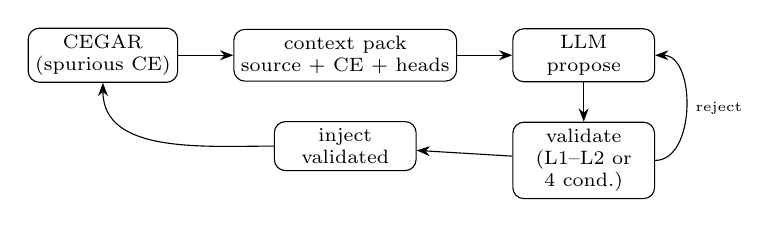
\begin{tikzpicture}[node distance=5mm and 7mm, >={Stealth[]},
  box/.style={draw, rounded corners, align=center, inner sep=2.5pt, font=\scriptsize,
              minimum width=18mm}]
  \node[box] (cegar) {CEGAR\\(spurious CE)};
  \node[box, right=of cegar] (pack) {context pack\\source + CE + heads};
  \node[box, right=of pack] (llm) {LLM\\propose};
  \node[box, below=of llm] (val) {validate\\(L1--L2 or\\4 cond.)};
  \node[box, below=of pack] (inject) {inject\\validated};
  \draw[->] (cegar)--(pack); \draw[->] (pack)--(llm); \draw[->] (llm)--(val);
  \draw[->] (val)--(inject); \draw[->] (inject.west) to[out=180,in=270] (cegar.south);
  \draw[->] (val.east) to[out=0,in=0] node[right,font=\tiny]{reject} (llm.east);
\end{tikzpicture}%
}
\caption{Engine-validated candidate provider loop (\Cref{tab:tiers}). Predicates: L1--L2;
ranking functions: four SMT conditions (\Cref{sec:rank}).}
\label{fig:pipeline}
\end{figure}

\paragraph{Context pack.} Three components: (i)~the stripped C source (global structure,
declarations, loop topology); (ii)~the spurious CE as an SMT-LIB2 block formula
$\varphi_1\wedge\cdots\wedge\varphi_k=\bot$ with SSA renaming, exposing concrete per-iteration
state; and (iii)~the CFA loop-head labels, which double as the only legal injection targets,
so hallucinated locations are rejected by construction.

\paragraph{Validation cascade.} Every proposed predicate must pass \textbf{L1 (contract)}
and \textbf{L2 (vocabulary)} or be silently discarded. L1 requires valid JSON, a recognised
loop-head key, and a syntactically valid C Boolean expression. L2 requires every free variable
to be in scope at the target loop head, killing the common ``undeclared variable'' hallucination.
We also implemented \textbf{L3 (SMT entailment)} for block-wise classification but do not use it:
ablation on \texttt{full\_scalar} favoured L1/L2-only injection, so all runs in \Cref{sec:eval} keep
L3 off. Survivors of L1/L2 are added to the PredicateCPA precision; adding predicates only refines the
abstraction, so the CEGAR soundness invariant is preserved unconditionally.

\paragraph{Configuration.} \tool{} uses \llm~\cite{deepseekv4} with chain-of-thought disabled (non-thinking
median latency $2.4$\,s vs.\ 50--90\,s for reasoning traces within a 300\,s budget).

\subsection{Ranking-Function Oracle (Termination)}
\label{sec:rank}

The same role transfers to termination with a different artifact. When lasso-based template
synthesis returns \textsc{Unknown} for a lasso, \tool{} asks the LLM for one or more candidate
ranking functions, each with an optional \emph{supporting invariant} $I$ (the LLM is told $f$
must be provably non-negative, and to supply the invariant that bounds it if needed). A
candidate $(f,I)$ is parsed into a linear integer term and certified against the lasso
transition relation $T(x,x')$ by four SMT unsatisfiability checks:
\begin{align*}
\text{initiation: } &\textit{Stem}\Rightarrow I(x_{\text{entry}}) &
\text{bounded: } &I(x)\wedge T(x,x')\Rightarrow f(x)\ge 0\\
\text{consecution: } &I(x)\wedge T(x,x')\Rightarrow I(x') &
\text{decrease: } &I(x)\wedge T(x,x')\Rightarrow f(x')<f(x)
\end{align*}
When $I=\mathit{true}$ the first two are trivial and this reduces to a pure ranking check. If
all four hold, $(f,I)$ \emph{soundly} proves the lasso terminates and is handed to the
termination engine exactly as a template-synthesised argument would be; otherwise the
candidate is discarded. Soundness is immediate and stronger than in the predicate case: $I$
is \emph{verified inductive} (not assumed), and a candidate for a genuinely non-terminating
lasso cannot pass the decrease check, so the oracle can never turn a non-terminating program
into \textsc{True}. The loop transition is read on the JavaSMT side of the lasso construction,
so the four checks run with no translation to the synthesiser's term representation.

\section{Evaluation}
\label{sec:eval}

\paragraph{Setup.} All runs use \cpa{} with \tool{} extensions, 300\,s per task (unless noted),
and \llm{} (non-thinking, temperature 0), at most five LLM rounds per predicate analysis
(schedule-gated). We report \emph{solved} tasks, PAR-2, and \emph{wrong} verdicts. Main safety:
SV-COMP Loops ReachSafety (764 tasks); \Cref{sec:generalisation} adds NoOverflow and termination.
\emph{Stock} = unmodified \cpa{}; \texttt{svcomp26} = competition portfolio in track~\emph{(ii)}.
Across every configuration below, \tool{} produced \textbf{zero wrong verdicts}; we omit a
wrong column and state soundness once here.

\subsection{ReachSafety Evaluation}
\label{sec:scheduling}

\Cref{tab:safety} has two tracks: \emph{(i)}~predicate worker in isolation (mechanism and
schedule decomposition); \emph{(ii)}~\texttt{svcomp26} portfolio (saturation and when-to-fire
deployment). The $\Delta$ column is cumulative within each track.

\paragraph{Firing schedule.} Orthogonal to \emph{which} predicates the oracle proposes is
\emph{when} it fires. On the isolated worker, the v1.7.1 default
(\texttt{every\_n\_or\_interval}, peel threshold~4) solves only 236 tasks ($+12$): peel
misfires on converging tasks whose CE trace crosses four loop-head visits
(\texttt{divbin}, \texttt{hard-u}). On the \texttt{svcomp26} portfolio (\Cref{tab:safety},
track~\emph{(ii)}), stock-first and peel pull in opposite directions: stock-first favours
converging proofs and time budget; peel favours early-divergence loops such as
\texttt{heapsort}---each recovers tasks the other misses. The design principle is \emph{fire
only when stock is not converging}, implemented as a \emph{stock-first} schedule (never at
refinement~\#1; otherwise after $K{=}10$ refinements or $D{=}15$\,s) and an optional \emph{peel}
trigger (refinement~\#2$+$ when loop-head visits $\ge 4$). Converging tasks peak at three visits;
diverging tasks cross four at refinement~\#2--\#4. Thresholds $K$, $D$, and the peel visit count
remain tunable (\Cref{sec:discussion}). \Cref{sec:casestudies} illustrates the trade-off on
\texttt{heapsort} and \texttt{nested-3}.

\begin{table}[t]
\caption{Loops ReachSafety results (764 tasks, 300\,s, 0 wrong). Two tracks; within a track only
the stated lever changes. $\Delta$ is cumulative over that track's baseline row.
\textsuperscript{a}Source-prior ablation (recorded run, 2026-06-17): PAR-2 from
\texttt{loops\_reachsafety\_unreach\_source\_prior\_loops}.
\textsuperscript{b}Schedule decomposition on the isolated worker (2026-06-22 controlled arms).
Track~\emph{(ii)} Steps~0--3: sequential \texttt{svcomp26-vguide} deployment
(\texttt{svcomp26\_deploy\_20260623}).}
\label{tab:safety}
\centering
\small
\begin{tabular}{@{}clccc@{}}
\toprule
Track & Configuration & Solved & $\Delta$ & PAR-2 (s) \\
\midrule
\multicolumn{5}{@{}l}{\emph{(i) Predicate oracle} --- \texttt{predicateAnalysis} in isolation} \\
 & stock (no oracle)                                    & 224 & --- & 428.4 \\
 & + oracle at refinement \#0 (source-prior; source only)\textsuperscript{a} & 224 & 0   & 427.1 \\
 & + oracle at \#1; \texttt{every\_n\_and\_interval}, peel=0 & \textbf{253} & +29 & 406.5 \\
 & + skip \#1 only; \texttt{every\_n\_or\_interval}, peel=0\textsuperscript{b} & 252 & +28 & 407.4 \\
 & + v1.7.1 default; \texttt{every\_n\_or\_interval}, peel=4\textsuperscript{b} & 236 & +12 & 418.8 \\
\addlinespace
\multicolumn{5}{@{}l}{\emph{(ii) \texttt{svcomp26} portfolio} --- progressive deployment; oracle on from Step~1} \\
 & Step 0: stock (no oracle)                            & 486 & --- & 222.5 \\
 & Step 1: + oracle, fire-at-\#1 (\texttt{every\_n\_and\_interval}, peel=0) & 493 & +7  & 217.9 \\
 & Step 2: + stock-first (skip \#1; $K{=}10$ / $D{=}15$\,s; peel=0) & \textbf{505} & +19 & 209.0 \\
 & Step 3: + peel (loop-head visits $\ge 4$)             & 505 & +19 & 211.3 \\
\bottomrule
\end{tabular}
\end{table}

Track~\emph{(i)}: fire-at-\#1 adds 29 solves ($224{\to}253$); source-prior at \#0 stays at 224,
so CE context drives the gain; v1.7.1 peel drops to 236 ($252{\to}236$). Track~\emph{(ii)}:
saturation limits Step~1 to $+7$ ($486{\to}493$). Stock-first (Step~2) adds $+12$
($493{\to}505$) with the best PAR-2 on this batch; peel (Step~3) keeps 505 solves but swaps nine
wins for nine losses---recovering \texttt{heapsort} and \texttt{nested9} while regressing tasks
such as \texttt{hard2} and \texttt{loopv2}---and raises PAR-2 slightly. Neither schedule
dominates; the two triggers are complementary and their balance can be retuned. Every predicate
still passes L1/L2.

\subsection{Case Studies}
\label{sec:casestudies}

\paragraph{A predicate win: \texttt{count\_up\_down-1}.} This is the running example of
\Cref{lst:example}. Stock predicate analysis discovers one conjunct per loop unrolling and times
out after 69 refinements. When the oracle fires at the first spurious CE, \tool{} proposes four predicates---$y=n-x$
(the relational invariant the example needs), $x\ge 0$, $y\le n$, and $x>0$; all four pass
L1/L2, and CEGAR then closes the proof in \textbf{2 refinements at 3.9\,s}---a 95\%
wall-time and 97\% refinement reduction from a single oracle call.

\paragraph{Why timing decides it: \texttt{heapsort} vs.\ \texttt{nested-3}.} These two tasks sit
on opposite sides of the scheduling trade-off. \texttt{heapsort} diverges under stock and needs an
\emph{early} call: the peel trigger fires at refinement~\#4, injecting index bounds
($1\le i,j,l\le n$) that close the proof; count/time-only stock-first arrives too late and the
analysis ends at \textsc{Unknown}. \texttt{nested-3} is the mirror: stock converges in 2
refinements, so firing at \#1 injects mutually exclusive facts ($\mathit{st}=0$ vs.\ $\mathit{st}=1$),
each accepted by L1/L2 but jointly noisy, and the proof blows up to a timeout---exactly what
stock-first avoids. A portfolio tuning therefore balances both levers rather than maximising one
alone (\Cref{tab:safety}, Steps~2--3).

\subsection{Generalisation}
\label{sec:generalisation}

\paragraph{NoOverflow (predicate oracle).} NoOverflow checking routes through the same
predicate-refinement hook as reachability---a config-only flip on the overflow predicate
component, with no Java or prompt changes. On \texttt{no\_overflow\_scalar} (452 tasks) under
the svcomp26 overflow portfolio, stock solves 362 and \tool{} solves 366 ($+4$). At a 120\,s
limit the lift was $+6$; two tasks stock catches up by 300\,s, leaving four sound
\tool{}-only wins.

\paragraph{Termination (ranking-function oracle).} When lasso-based template synthesis returns
\textsc{Unknown}, the LLM proposes ranking functions validated by the four-condition check of
\Cref{sec:rank}. On \texttt{termination\_scalar} (146 integer-termination tasks, lasso route in
isolation): stock solves 80; with the oracle, 84 ($+4$, \textbf{0 lost}). The four new solves are
SMT-validated measures outside the template family, e.g.\ $f=n-i$, $f=k-i$, $f=x$, and
$f=y_1+y_2$ with $I=(y_1>0\wedge y_2>0)$. Stock solves the same 80 at 60\,s and 300\,s, so
residual failures are template-\emph{unsolvable}, not time-limited.

\begin{table}[t]
\caption{Generalisation beyond Loops ReachSafety (300\,s, 0 wrong). Termination: lasso analysis
in isolation.}
\label{tab:generalisation}
\centering
\begin{tabular}{llcc}
\toprule
Property & Benchmark (tasks) & Stock & + \tool{} \\
\midrule
NoOverflow & \texttt{no\_overflow\_scalar} (452) & 362 & \textbf{366} (\,+4\,) \\
Termination & \texttt{termination\_scalar} (146) & 80 & \textbf{84} (\,+4\,) \\
\bottomrule
\end{tabular}
\end{table}

\section{Discussion and Limitations}
\label{sec:discussion}

\paragraph{Sound predicates can still be noisy hints.} L1/L2 guarantee syntactic validity, not
usefulness (\Cref{sec:casestudies}, \texttt{nested-3}). The divergence-aware schedule avoids
firing on converging stock proofs; a mutual-consistency check across injected predicates would
help further, at extra SMT cost.

\paragraph{Portfolio vs.\ isolation.} The oracle adds 29 solves in isolation but only $+7$ after
naive portfolio deployment ($486{\to}493$). Stock-first reaches 505 ($+19$ vs.\ stock) with the
best PAR-2 here; peel at the same solve count exchanges early-divergence wins for other portfolio
proofs (\texttt{heapsort}/\texttt{nested9} vs.\ \texttt{hard2}/\texttt{loopv2}). \emph{When} to
fire is decisive in isolation and remains a tunable trade-off in portfolio deployment---$K$, $D$,
and the peel visit threshold are not yet jointly optimised for this benchmark.

\paragraph{The reachability gain is also bounded.} Of the remaining unsolved tasks, roughly 70\%
are \emph{nonlinear-arithmetic} instances (the SV-COMP \texttt{nla-digbench} family)---e.g.\
\texttt{cohencu} asserts $x=n^3$ and $y=3n^2{+}3n{+}1$---outside a linear predicate engine.
Further reachability gains need nonlinear invariant synthesis or a new injection point; schedule
knobs may still be refined for specific task families but are no longer a free large increment.

\paragraph{The termination gain has a small, characterised ceiling.} On the 56 stock-\textsc{Unknown}
terminating tasks, the oracle fires on 9 (winning 4); \textbf{40 never produce a lasso}---pointer/array/string
loops where the safety analysis gives up first. Three cheap levers on the tasks that do fire
\emph{none helped} (prompt tweak $4{\to}3$; verify-and-repair $+0$; stem-formula context $4{\to}2$).
Portfolio-net gain is $\le 4$ because a parallel termination-to-safety worker has no LLM path.

\paragraph{Online LLM dependency and \textsc{False}-path blindness.} Live re-runs need an API
key; competition submission would need a local model or candidate cache. Both oracles improve only
\textsc{True} counts; extending to \textsc{False} needs a different artifact---a concrete violating
input validated by execution rather than an SMT proof (\Cref{sec:future}).

\section{Related Work}
\label{sec:related}

\paragraph{LLM loop invariants and verification.}
Early work asks whether LLMs can predict invariants at all~\cite{pei2023}.
Subsequent systems combine generation with formal checking in a propose-and-repair loop:
Lemur~\cite{lemur2024} presents a sound proof calculus where an LLM proposes sub-goals checked by
automated reasoners; LORIS~\cite{loris2026} refines invariants via feedback on local reasoning
errors in failed verification conditions; Quokka~\cite{quokka2025} provides a simple, sound
evaluation procedure for LLM-generated invariants on an SV-COMP-scale benchmark; and hybrid
LLM+SMT frameworks~\cite{loopinvariant2025,neuroinv2025} target Code2Inv-style synthesis with
weakest-precondition or solver-guided refinement.
These tools are largely \emph{standalone} synthesizers or front-ends: they generate invariants
(or contracts) and check them, but do not inject candidates into a running CEGAR engine's
abstraction refinement loop.
\tool{} instead hooks the predicate worker inside \cpa{}: spurious-CE context, L1/L2 gating, and
precision-only injection at loop heads (\Cref{sec:pred}).

\paragraph{Counterexample-guided and compositional LLM verification.}
CIll~\cite{cill2026} is closest in spirit on the \emph{counterexample} axis: it refines LLM
invariant candidates from counterexamples to induction (CTIs) in hardware model checking.
ConVer~\cite{conver2026} composes top-down contract synthesis with a CEGAR--CEGIS loop for C
programs; IC3+LLM work~\cite{ic3llm2026} targets distributed protocols rather than software CEGAR.
Clover~\cite{clover2024} closes the loop between code, docstrings, and Dafny annotations via
consistency checking---a different artifact, but the same ``LLM proposes, formal tool gates''
pattern.
Neuro-symbolic proof generation~\cite{neurosymbolic2026} scales interactive verification with LLM
hints, and agentic model checking~\cite{agenticmc2026} wraps exploration in an autonomous LLM
loop; \tool{} is deliberately lighter---structured Tier~S oracle calls under artifact-specific
gates, without replanning or trusting LLM verdicts.

\paragraph{Positioning.}
Against this landscape, our distinguishing points are: (i)~embedding in \cpa{} CEGAR rather than
standalone synthesis; (ii)~a single engine-validated candidate-provider role for \emph{both}
predicates (L1/L2) and ranking functions (four-condition SMT); and (iii)~empirical evidence that
\emph{when} the oracle fires matters as much as \emph{what} it proposes, with different optimal
schedules in isolation versus competition portfolio deployment (\Cref{tab:safety}).

\section{Conclusion}
\label{sec:concl}

\tool{} integrates an LLM into \cpa{} as an engine-validated candidate provider---propose, validate,
decide---covering safety predicates and termination ranking functions with zero wrong verdicts in
every configuration we report. On Loops ReachSafety the predicate oracle adds 29 solves in isolation
($224{\to}253$) but only $+7$ under portfolio saturation ($486{\to}493$); stock-first reaches 505
($+19$), while peel offers a complementary win/loss trade-off at the same solve count. Residual tasks
are dominated by nonlinear arithmetic; termination
and NoOverflow each add four sound solves with characterised ceilings. An artifact with source,
configurations, benchmark lists, recorded outputs, and scripts is publicly
available;\footnote{Archived at \url{https://doi.org/10.5281/zenodo.20745141}; development
repository at \url{https://github.com/swear01/cpachecker}.} all tables regenerate offline.

\section{Future Work}
\label{sec:future}

Earlier termination injection for pointer/array/string loops; nonlinear invariant synthesis or a new
safety injection point; joint calibration of stock-first ($K$, $D$) and peel thresholds on portfolio
benchmarks; execution-validated bug witnesses for \textsc{False}; and a local or distilled
model for competition submission.

\bibliographystyle{splncs04}
\bibliography{references}

\end{document}
